% !TeX spellcheck = nb_NO
% Kommentaren ovenfor gir instruks til editoren din om at den skal bruke norsk stavekontroll. Dette fungerer bl.a. i TeXstudio.

\documentclass[a4paper,norsk]{article}
% Norsk orddeling
\usepackage[norsk]{babel}
% AMS-pakkene er nyttige
\usepackage{amsmath,amsfonts,amssymb,amsthm}
% For å definere lister, som f.eks. deloppgaver
\usepackage{enumitem}
% Inneholder mye nyttig, slik som \coloneqq
\usepackage{mathtools}
% Penere kalligrafiske fonter
\usepackage[utf8]{inputenc}
\usepackage[T1]{fontenc}
\usepackage[a4paper, margin=0.5in]{geometry}
\usepackage{mathabx}
\usepackage{amsthm}
\usepackage{listings}
\usepackage{xcolor}
\usepackage{ifthen}
\usepackage{hyperref}


\setcounter{secnumdepth}{2}  % Sections and subsections numbered

% Python style  
\lstdefinestyle{pythonstyle}{
    language=Python,
    basicstyle=\ttfamily\small,
    keywordstyle=\color{blue},
    commentstyle=\color{green},
    numbers=left,
    frame=single
}

% Bruk bedre symboler for ≥, ≤, epsilon og phi
\renewcommand{\geq}{\geqslant}
\renewcommand{\leq}{\leqslant}
\newcommand{\eps} {\varepsilon}
\renewcommand{\epsilon}{\varepsilon}
\renewcommand{\phi}{\varphi}

% Definer de vanligste mengdene og funksjonene
\newcommand{\R}{\mathbb{R}}
\newcommand{\K}{\mathbb{K}}
\newcommand{\C}{\mathbb{C}}
\newcommand{\N}{\mathbb{N}}
\newcommand{\Z}{\mathbb{Z}}
\newcommand{\Q}{\mathbb{Q}}
% \L er definert som noe annet fra før av, så vi må redefinere \L
\renewcommand{\L}{\mathcal{L}}
% Rommet av polynomer
\newcommand{\Pol}{{\mathcal{P}}}
\DeclareMathOperator{\id}{id}
\DeclareMathOperator{\Image}{im}
\DeclareMathOperator{\Kernel}{ker}
\DeclareMathOperator{\Span}{span}
\DeclareMathOperator{\Rank}{rank}
\DeclareMathOperator{\Diag}{diag}
\DeclareMathOperator{\Proj}{proj}
\newcommand{\basis}{{\mathcal{B}}}
\newcommand{\basiss}{{\mathcal{C}}}
\newcommand{\basisss}{{\mathcal{D}}}
\newtheorem*{theorem}{Theorem}
\newtheorem*{corollary}{Corollary}
\newtheorem*{lemma}{Lemma}
\newtheorem*{definition}{Definition}
\newtheorem*{proposition}{Proposisjon}

\usepackage[most]{tcolorbox}
\newtcolorbox{algoritme}[1]{
  title=Algoritme~#1,
  colback=white,
  colframe=black,
  boxrule=0.5pt,
  arc=2mm,
  left=3mm,
  right=3mm,
  top=1mm,
  bottom=1mm
}



% Definer oppgavemiljøet
\newenvironment{oppgave}[1]%
	{\trivlist{}\item\relax\textbf{Løsning på #1.}\medspace}%
	{\endtrivlist}
% Deloppgavelister
\newlist{deloppgave}{enumerate}{1}
\setlist[deloppgave,1]{label=(\textbf{\alph*}),align=left}

\title{Oblig 4 \\ MAT1125, høst 2025}
\author{Oliver Ekeberg}
\begin{document}
\maketitle

\tableofcontents

\section*{6.1 Overblikk og generelle ideer}
\addcontentsline{toc}{section}{6.1 Overblikk og generelle ideer}

En sinusbølge karakteriseres ved \textbf{\textit{frekvens}} og \textbf{\textit{amplitude}}. Vi skal her undersøke om en generell funksjon kan uttrykkes ved hjelp av sinusbølger. Spesielt på formen

\[
    sin(kt)
\]
for $ t \in \mathbb{R} $ og $ k \in \mathbb{Z} $. Kan vi uttrykke en generell funksjon $ f: \mathbb{R} \rightarrow \mathbb{R} $ som
\[
    f(t) = \sum_{ k \in \mathbb{N} }^{  } c_k sin(kt) 
\]

for $ t \in \mathbb{R} $ og $ c_k \in \mathbb{R} $? Vi kan utvide til en funksjon på formen

\[
    f(t) = \sum_{ k \in \mathbb{N} }^{  } c_k sin(kt) + \sum_{ k \in \mathbb{N}_0 }^{  } d_k cos(kt)
\]
for $ t \in \mathbb{R} $. Vi gjør en videre antagelse, nemlig at f er $ 2\pi $ perdiodisk,
\[
    f(t + 2\pi) = f(t) \forall t
\]

Vi spør også om vi kan uttrykke en generell $ 2\pi $ periodisk funksjon $ f: \mathbb{R} \rightarrow \mathbb{C} $ som
\[
    f(t) = \sum_{ k \in \mathbb{N} }^{  } c_k sin(kt) + \sum_{ k \in \mathbb{N}_0 }^{  } d_k cos(kt)
\]
hvor $ c_k, d_k \in  \mathbb{C} $. Dette er svært tungt, men vi kan bruke Eulers formel
\[
    e^{it} = \cos(t) + \sin(t)
\]
og vi forenkler uttrykket til
\[
    f(t) = \sum_{ k \in \mathbb{Z} }^{  } \hat{f}_k e^{it}
\]
for $ t \in  \mathbb{R} $ og $ \hat{f}_k \in \mathbb{C} $ 


\begin{oppgave}{6.1.1}
Vis at de to uttrykkene er ekvivalente om $ \hat{f}_k $  velges som

\[
    \hat{f}_k = \begin{cases}
      \frac{ c_k }{ 2i } + \frac{ d_k }{ 2 } \text{ for $ k > 0 $ }\\ 
      d_0 \text{ for $ k=0 $ }\\
      \frac{ -c_{-k} }{ 2i } + \frac{ d_{-k} }{ 2 } \text{ for $ k< 0 $ }
    \end{cases}
\]

\begin{proof}{6.1.1}
Vi begynner med å forme uttrykket på kompleks form

\begin{align*}
  \sum_{ k \in \mathbb{Z} }^{  } \hat{f}_k e^{ikt} &= d_0 + \sum_{ k \in \mathbb{Z} }^{  } \hat{f}_k e^{ikt} + \hat{f}_{-k} e^{-ikt}
\end{align*}

Jeg omgrupperer uttrykket litt.

\begin{align*}
  \sum_{ k \in \mathbb{Z} }^{  } \hat{f}_k e^{ikt} &= \sum_{ k \in \mathbb{Z} }^{  }  \left( \frac{ c_k }{ 2i } + \frac{ d_k }{ 2 } \right) \left( \cos(kt) + i \sin(kt) \right) \\
  &= \sum_{ k \in \mathbb{Z} }^{  } \frac{ c_k }{ 2i } \cos(kt) + \frac{ c_k }{ 2 } \sin(kt) + \frac{ d_k }{ 2 } \cos(kt) + \frac{i d_k }{ 2 } \sin(kt) 
\end{align*}

Det andre uttrykket i summen er da

\begin{align*}
  \sum_{ k \in \mathbb{Z} }^{  } \hat{f}_{-k} e^{-ikt} &= \sum_{ k \in \mathbb{Z} }^{  } \left( \frac{ -c_{-k} }{ 2i } + \frac{ d_{-k} }{ 2 }  \right) \left( \cos(kt) - i \sin(kt) \right) \\
  &= \sum_{ k \in \mathbb{Z} }^{  }  - \frac{ c_{-k} }{ 2i } \cos(kt) + \frac{ c_{-k} }{ 2 } \sin(kt) + \frac{ d_{-k} }{ 2 } \cos(kt) - \frac{ i d_{-k}  }{ 2 }  \sin(kt) 
\end{align*}

Legg sammen uttrykkene og få

\begin{align*}
  d_0 + \sum_{ k \in \mathbb{Z} }^{  } \hat{f}_k e^{ikt} + \hat{f}_{-k} e^{-ikt} &= d_0 + \sum_{ k \in \mathbb{Z} }^{  } \frac{ c_k }{ 2i } \cos(kt) + \frac{ c_k }{ 2 } \sin(kt) + \frac{ d_k }{ 2 } \cos(kt) + \frac{i d_k }{ 2 } \sin(kt)\\ 
  &- \frac{ c_{-k} }{ 2i } \cos(kt) + \frac{ c_{-k} }{ 2 } \sin(kt) + \frac{ d_{-k} }{ 2 } \cos(kt) - \frac{ i d_{-k}  }{ 2 }  \sin(kt) 
\end{align*}

Siden for $ k < 0 $ så er $$ \hat{f}_{-k} = \frac{ -c_{-k} }{ 2i } + \frac{ d_{-k} }{ 2 } = \frac{ -c_k }{ 2i } + \frac{ d_k }{ 2 } $$, så kan vi kansellere de komponentene med komplekse verdier i seg.
\begin{align*}
  d_0 + \sum_{ k \in \mathbb{Z} }^{  } \hat{f}_k e^{ikt} + \hat{f}_{-k} e^{-ikt} &= d_0 + \sum_{ k \in \mathbb{Z} }^{  } c_k \left( \frac{ 1 }{ 2 } \sin(kt) + \frac{ 1 }{ 2 } \sin(kt)  \right) + d_k \left( \frac{ 1 }{ 2 } \cos(kt) + \frac{ 1 }{ 2 } \cos(kt) 
 \right) \\
 &= d_0 + \sum_{ k \in \mathbb{Z} }^{  } c_k \sin(kt) + d_k \cos(kt)  
\end{align*}
\end{proof}
\end{oppgave}


\begin{definition}{6.1.2}
For $ f, g : \left[ 0, 2\pi \right) \rightarrow \mathbb{C} $ definerer vi $ L^2 $ indreproduktet som 
\[
    \langle f, g,  \rangle_{ L^2 } = \frac{ 1 }{ 2\pi } \int_{0}^{2\pi}  f(t) \overline{g(t)}dt
\]
\end{definition}

\begin{oppgave}{6.1.3}
  Vis at $ \left( e_k \right) _{k \in \mathbb{Z}} $ er en ortonormal liste med hensyn på indreproduktet $ \langle *, * \rangle_{ L^2 }  $. altså at
  \[
      \langle e_j, e_k \rangle_{ L^2 } = \delta_{jk} \forall j, k \in \mathbb{Z}
  \]
\begin{proof}{6.1.3}
\begin{align*}
  \langle e_j, e_k \rangle_{ L^2 } &= \frac{ 1 }{ 2\pi } \int_{0}^{2\pi} e_j \cdot e_k dt \\
  &= \frac{ 1 }{ 2\pi } \int_{0}^{2\pi} e^{ikt} e^{-ijt} \\
  &= \frac{ 1 }{ 2\pi } \int_{0}^{2\pi} e^{ikt} e^{-ijt} \\
  &= \frac{ 1 }{ 2\pi } \int_{0}^{2\pi} \delta_{jk} dt  \\
  &= \delta_{jk} \frac{ 1 }{ 2\pi } \int_{0}^{2\pi} dt \\
  &= \delta_{jk} \left( 2 \pi - 0 \right)  \\
  &= \delta_{jk}
\end{align*}
Dette får vi fordi 
\[
    e^{ikt} e^{-ijt} = \begin{cases}
      e^0, \text{ for $ k=j $ }\\
      e^{ikt} e^{-ijt} \neq e^0, \text{ for $ k\neq j $ }
    \end{cases}
\]


\begin{align*}
  \frac{ 1 }{ 2\pi } \int_{0}^{2\pi} e^{ikt} e^{-ijt} dt &= \frac{ 1 }{ 2\pi } \int_{0}^{2\pi} e^{ it \left( k - j \right)  }  dt \\
  &= \frac{ 1 }{ 2\pi }  \left[ \frac{ e^{ it \left( k - j \right)  } }{ i \left( k - j \right)  } \right]_0^{2\pi}\\
  &= \frac{ 1 }{ 2\pi } \left[ \frac{ e^{i2\pi \left( k - j \right)  } - 1}{ i \left( k-j \right)  } \right] 
\end{align*}

Vi kan nå vise at $ e^{i 2\pi k} = 1, \forall k \in  \mathbb{Z}$ 

\begin{center}
    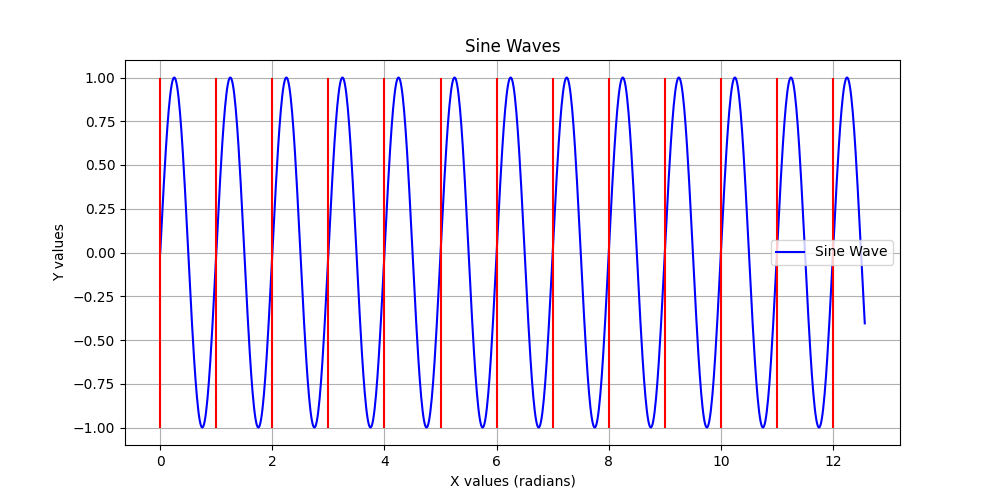
\includegraphics[width=0.9\textwidth,height=0.7\textheight,keepaspectratio]{figurer/sin_waves_exc_613.png}
\end{center}
\begin{center}
    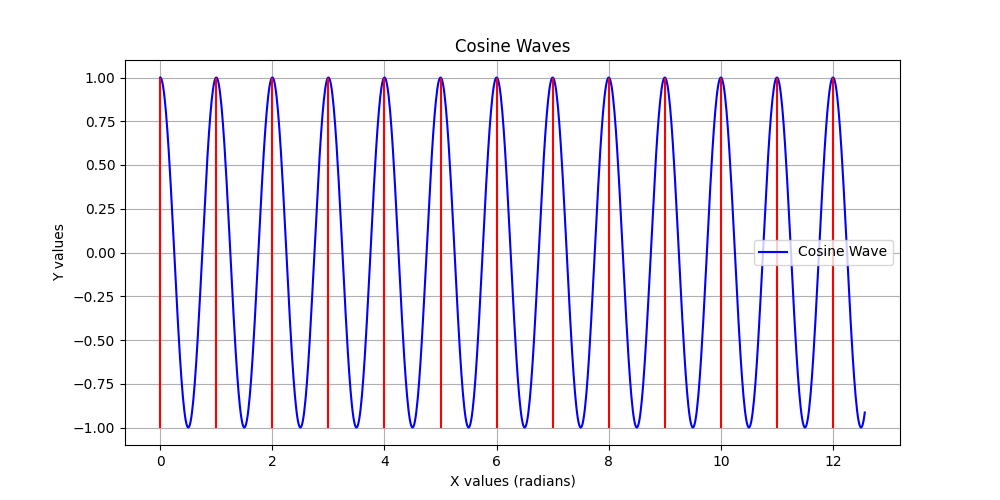
\includegraphics[width=0.9\textwidth,height=0.7\textheight,keepaspectratio]{figurer/cos_waves_exc_613.png}
\end{center}

siden $ k-j  \in \mathbb{Z}$ så vil $ e^{i 2\pi \left( k -j \right) } = 1 $ når $ k \neq j $  og vi får at $ \langle e_k, e_j \rangle_{ L^2 } = 0  $ for $ k\neq j $ og $ \langle e_k, e_j \rangle_{ L^2 } = 1  $ for $ k = j $. dermed er $ \langle e_k, e_j \rangle_{ L^2 } = \delta_{jk}  $ Det integrerte uttrykket $ \frac{ 1 }{ 2\pi } \left[ \frac{ e^{i2\pi \left( k - j \right)  } - 1}{ i \left( k-j \right)  } \right]  $ gjelder bare for når $ k \neq j $. Når $ k=j $, så får vi
\[
    \langle e_k, e_k \rangle_{ L^2 }  = \frac{ 1 }{ 2\pi } \int_{0}^{2\pi} e^{ikt} e^{-ikt}dt = \frac{ 1 }{ 2\pi } \int_{0}^{2\pi} e^0 dt = \frac{ 1 }{ 2\pi } \left[ 2\pi - 0 \right]   = 1
\]
\end{proof}   
\end{oppgave}



\section*{6.2 Moduloregning og periodiske funksjoner}
\addcontentsline{toc}{section}{6.2 Moduloregning og periodiske funksjoner}

La $ s, t \in \mathbb{R} $. Vi skriver
\[
    s = t \text{ mod } a
\]
hvis $ \exists $ en $ k \in \mathbb{Z} $ s.a. $ s = t+ ak $. Vi skal spesielt studere tilfellet der $ s = s + 2\pi = s + 4 /pi = ... mod 2\pi $ 
Om vi ser på s som en vinkel på enhetssirkelen, så er det analogt med å se på modulo som ekstra omdreining som ender på samme punkt. Punktenen på enhetssirkelen danner en \textbf{\textit{gruppe}} $ \mathbb{T} $ \\

En gruppe er et "rom" hvor vi kan addere og subtrahere, men ikke nødvendigvis multiplisere eller dividere. Om $ s = s' \text{ mod } 2\pi$ og $ t = t' \text{ mod } 2\pi $ er $ s = s' + 2\pi j $ og $ t = t' + 2\pi k $ for $ j, k \in \mathbb{Z} $

\[
    s + t = s' + t' + 2\pi \left( j + k \right) 
\]
så $ s + t = s' + t' \text{ mod } 2 \pi $. Vi kan beregne avstanden på $ \mathbb{T} $
\[
    \left|  s - t \right| := min \left\{ \left| s - t - 2\pi k \right| : k in
    \mathbb{Z}  \right\} 
\]

\begin{definition}{6.2.1}
En funksjon $ f : \mathbb{R} \rightarrow \mathbb{C} $ er \textbf{\textit{periodisk}} om $ \exists $ en $ a > 0 $ s.a. 
\[
    f(s + a) = f(s) \forall s \in \mathbb{R}
\]
Tallet a er \textbf{\textit{perioden}} 
\end{definition}

\begin{oppgave}{6.2.2}
Vis at om f er periodisk med periode am så er også $ f(s + ak) = f(s) \forall k \in \mathbb{Z} $ 

\begin{proof}{6.2.2}
Her er det nyttig å bruke induksjon
\begin{itemize}
  \item Viser først at for $ P_0 $ er $ f(s + a \cdot 0) = f(s + 0) = f(s) $  
  \item For $ P_1 $ er $ f(s + a \cdot 1) = f(s+a) = f(s) $  er sant av definisjonen til en periodisk funksjon
  \item Anta at $ P_k $  er sann for en $ k \geq 1 $. Hypotesen er at $ f(s + ak) = f(s)  $ for en $ k \in \mathbb{Z} $ 
  \item Vil vise at $ P_{k+1}: f(s + a \left( k+1 \right) ) = f(s) $
  \begin{align*}
    f(s + a \left( k+1 \right)) &= f( \left( s + ak \right) + a) \\
    &=   f \left( s + ak \right) \text{ Dette kommer av definosjonen til en periodisk funksjon } f(s+a) = f(s) \\
    &= f \left( s + ak \right) = f(s) \text{ Her bruker vi hypotesen vår} 
  \end{align*}
  
\end{itemize}
\end{proof}
\end{oppgave}
 
\begin{oppgave}{6.2.3}
La $ k \in \mathbb{Z} $. Vis at funksjonene 
\begin{itemize}
  \item $ f_k(t) := e^{ikt} $
  \item $ g_k(t) := \cos(kt)   $  
  \item $ h_k(t) := \sin(kt)  $ 
\end{itemize}
er $ 2\pi $ periodiske


\begin{proof}{6.2.3}
\begin{itemize}
  \item Vi begynner med $ f_k(t) = e^{ikt} $. Må vise at 
  \[
      f_k(t+ 2\pi) = f_k(t) \rightarrow e^{ik \left( t + 2\pi \right) } = e^{ikt}
  \]

  \begin{align*}
    e^{ik \left( t + 2\pi \right) } &= e^{ikt} e^{ik2\pi}
  \end{align*}
  \[
      e^{ik2\pi}  = \cos(k2\pi)  + i \sin(k2\pi) 
  \]
  Vi vet at $ \cos(k 2\pi)   $ for en $ k \in \mathbb{Z} $ gir $ \cos(k 2\pi) =1  \forall k \in \mathbb{Z}$ og at $ \sin(2k \pi) = 0 \forall k \in \mathbb{Z}  $. Dermed er
  \[
      e^{ik2\pi} = 1 \forall k \in  \mathbb{Z}
  \]
  Dermed er 
  \begin{align*}
    e^{ik \left( t + 2\pi \right) } &= e^{ikt} e^{ik2\pi}\\
    &= e^{ikt} \cdot 1\\
    &= e^{ikt}
  \end{align*}
  og jeg har vist at $ f_k(t) = e^{ikt} $  er en periodisk funksjon
  \item Vi har nå $ g_k(t) = \cos(kt)   $. Skal så vise at $ \cos(k \left( t+2\pi \right) ) = \cos(kt)     $. 
  \[
      \cos(kt)  = \frac{ e^{ikt} + e^{-ikt}  }{ 2 }
  \]
  Dermed blir 
  \begin{align*}
    \cos(k \left( t + 2\pi \right) )  &= \frac{ e^{ik \left( t + 2\pi \right) } + e^{-ik \left( t + 2 \pi  \right) }   }{ 2 }\\
    &= \frac{ e^{ikt} e^{ik2 \pi } + e^{-ikt} e^{-ik2 \pi }   }{ 2}\\
    &= \frac{ e^{ikt} \cdot 1 + e^{-ikt} \cdot 1 }{ 2 } \\
    &= \frac{ e^{ikt} + e^{-ikt}  }{ 2 } \\
    &= \cos(kt)  
  \end{align*}
  
  \item Og nå tar vi siste $ h_k(t) = \sin(kt)  $. Skal vise at $ \sin(k \left( t + 2 \pi  \right) ) = \sin(kt)   $. Har oppgitt at
  \[
      \sin(kt) = \frac{ e^{ikt} - e^{-ikt}  }{ 2i }
  \]
  
  
  \begin{align*}
    \sin(k \left(  t + 2 \pi  \right) ) &= \frac{ e^{ik \left( t + 2 \pi  \right) - e^{-ik \left( t + 2 \pi  \right) }  }  }{ 2i }\\
    &= \frac{ e^{ikt} e^{ik2 \pi } - e^{-ikt} e^{-ik 2 \pi } }{ 2i}\\
    &= \frac{ e^{ikt} \cdot 1 - e^{-ikt} \cdot 1 }{ 2i }\\
    &= \frac{ e^{ikt} - e^{-ikt}  }{ 2i }\\
    &= \sin(kt) 
  \end{align*}
\end{itemize}
Det er greit å forklare at $ e^{-ikt} = 1  \forall k \in \mathbb{Z}$ fordi du kan bare gå bakover i negativ vinkelretning på enhetssirkelen
\end{proof}
\end{oppgave}  

\begin{oppgave}{6.2.10}
Finn fourierrekkene til følgende funksjoner
\begin{itemize}
  \item a) $ f: \mathbb{T} \rightarrow \mathbb{R} $ gitt ved $ f(t) = 1 $  
  \item b) $ f: \mathbb{T} \rightarrow \mathbb{R} $ gitt ved $ f(t) = t^2 $ for $ t \in \left[ -\pi, \pi \right)  $   
  \item c) $ f: \mathbb{T} \rightarrow \mathbb{R} $ gitt ved $ f(t) = e^{t}  $ for $ t \in \left[ 0, 2 \pi \right) $ 
\end{itemize}


\begin{proof}{6.2.10 a)}
Vi finner fourier rekken ved å finne fourier koeffisientene
\[
    \hat{f}_k = \langle f, e_k \rangle_{ L^2 } 
\]
og setter de inn i den generelle formen
\[
    f(t) = \sum_{ k =-n }^{ n } \hat{f}_k e_k
\]
\begin{align*}
  \hat{f}_k &= \frac{ 1 }{ 2 \pi } \int_{0}^{2 \pi 
  } e_0 \overline{e_k} dt \\
  &= \frac{ 1 }{ 2 \pi  }  \int_{0}^{2 \pi } e^{-ikt} dt \\  
  \frac{ 1 }{ 2 \pi  } \int_{0 }^{2 \pi } e^{-ikt} dt &=   \frac{ 1 }{ 2 \pi  } \left[ \frac{ -1 }{ ik } e^{-ikt}  \right]  _0^{2 \pi } \\
  &= \frac{ -1 }{ ik 2 \pi  } \left[ e^{-ik2 \pi } - 1  \right] \\
  &= 0
\end{align*}

Jeg bruker at $ f(t) = e_0 $ fordi det er den nærmeste projeksjonen av f ned på den ortonormale basises $ \left( e_k \right) _{k \in \mathbb{Z}} $. Dette er fordi $ e_0 = e^{ik \cdot 0} = 1 = f(t)  $\\

Så fourierrekken er \[
    f(t) = 1
\]

\end{proof}

\begin{proof}{6.2.10 b)}


Vi bruker det ortonormale basiset $e_k(t) = e^{ikt}$, $k \in \mathbb{Z}$, med indreprodukt:
\[
\langle f, g \rangle = \frac{1}{2\pi} \int_{-\pi}^{\pi} f(t) \overline{g(t)}  dt
\]

Fourier-koeffisientene er gitt ved:
\[
\hat{f}(k) = \langle f, e_k \rangle = \frac{1}{2\pi} \int_{-\pi}^{\pi} t^2 e^{-ikt}  dt
\]

Utregning av koeffisienter

\paragraph{Tilfelle $k = 0$:}
\[
\hat{f}(0) = \frac{1}{2\pi} \int_{-\pi}^{\pi} t^2  dt 
= \frac{1}{2\pi} \left[ \frac{t^3}{3} \right]_{-\pi}^{\pi}
= \frac{1}{2\pi} \cdot \frac{\pi^3 - (-\pi)^3}{3}
= \frac{1}{2\pi} \cdot \frac{2\pi^3}{3}
= \frac{\pi^2}{3}
\]

\paragraph{Tilfelle $k \neq 0$:}
La $I = \int_{-\pi}^{\pi} t^2 e^{-ikt}  dt$. Integrerer ved deler:
\begin{align*}
\text{La: } & u = t^2, \quad dv = e^{-ikt}dt \\
& du = 2tdt, \quad v = \frac{e^{-ikt}}{-ik}
\end{align*}
\begin{align*}
I &= \left[ t^2 \cdot \frac{e^{-ikt}}{-ik} \right]_{-\pi}^{\pi} 
   - \int_{-\pi}^{\pi} \frac{e^{-ikt}}{-ik} \cdot 2t  dt \\
&= \frac{-1}{ik} \left[ t^2 e^{-ikt} \right]_{-\pi}^{\pi} 
   + \frac{2}{ik} \int_{-\pi}^{\pi} t e^{-ikt}  dt
\end{align*}

Grensebidrag:
\[
\left[ t^2 e^{-ikt} \right]_{-\pi}^{\pi} = \pi^2 e^{-ik\pi} - \pi^2 e^{ik\pi} 
= \pi^2(e^{-ik\pi} - e^{ik\pi}) = \pi^2(-2i\sin(k\pi)) = 0
\]
siden $\sin(k\pi) = 0$ for $k \in \mathbb{Z}$.

Dermed:
\[
I = \frac{2}{ik} \int_{-\pi}^{\pi} t e^{-ikt}  dt
\]

Integrerer $\int t e^{-ikt}  dt$ ved deler:
\begin{align*}
\text{La: } & u = t, \quad dv = e^{-ikt}dt \\
& du = dt, \quad v = \frac{e^{-ikt}}{-ik}
\end{align*}
\begin{align*}
\int_{-\pi}^{\pi} t e^{-ikt}  dt &= \left[ t \cdot \frac{e^{-ikt}}{-ik} \right]_{-\pi}^{\pi} 
- \int_{-\pi}^{\pi} \frac{e^{-ikt}}{-ik}  dt \\
&= \frac{-1}{ik} \left[ t e^{-ikt} \right]_{-\pi}^{\pi} 
+ \frac{1}{ik} \int_{-\pi}^{\pi} e^{-ikt}  dt
\end{align*}

Grensebidrag:
\[
\left[ t e^{-ikt} \right]_{-\pi}^{\pi} = \pi e^{-ik\pi} - (-\pi)e^{ik\pi} 
= \pi(e^{-ik\pi} + e^{ik\pi}) = 2\pi\cos(k\pi)
\]

Integralet:
\[
\int_{-\pi}^{\pi} e^{-ikt}  dt = \left[ \frac{e^{-ikt}}{-ik} \right]_{-\pi}^{\pi} 
= \frac{e^{-ik\pi} - e^{ik\pi}}{-ik} = \frac{-2i\sin(k\pi)}{-ik} = 0
\]

Dermed:
\[
\int_{-\pi}^{\pi} t e^{-ikt}  dt = \frac{-1}{ik} \cdot 2\pi\cos(k\pi) = \frac{-2\pi\cos(k\pi)}{ik}
\]

Setter inn i $I$:
\[
I = \frac{2}{ik} \cdot \frac{-2\pi\cos(k\pi)}{ik} 
= \frac{-4\pi\cos(k\pi)}{i^2 k^2} 
= \frac{-4\pi\cos(k\pi)}{-k^2} 
= \frac{4\pi\cos(k\pi)}{k^2}
\]

Fourier-koeffisient for $k \neq 0$:
\[
\hat{f}(k) = \frac{1}{2\pi} \cdot I = \frac{1}{2\pi} \cdot \frac{4\pi\cos(k\pi)}{k^2} 
= \frac{2\cos(k\pi)}{k^2}
\]

Resultatet blir så

Fourier-koeffisienter:
\[
\hat{f}(k) = 
\begin{cases}
\dfrac{\pi^2}{3}, & k = 0 \\[1em]
\dfrac{2\cos(k\pi)}{k^2}, & k \neq 0
\end{cases}
\]

Fourier-rekke (kompleks form):
\[
t^2 \sim \sum_{k=-\infty}^{\infty} \hat{f}(k)e^{ikt} 
= \frac{\pi^2}{3} + \sum_{\substack{k=-\infty \\ k \neq 0}}^{\infty} \frac{2\cos(k\pi)}{k^2} e^{ikt}
\]
\end{proof}

\begin{proof}{6.2.10 c)}


Fourier-rekke for $f(t) = e^t$ på $[-\pi,\pi)$

Vi bruker det ortonormale basiset $e_k(t) = e^{ikt}$, $k \in \mathbb{Z}$, med indreprodukt:
\[
\langle f, g \rangle = \frac{1}{2\pi} \int_{-\pi}^{\pi} f(t) \overline{g(t)}  dt
\]

Fourier-koeffisientene er gitt ved:
\[
\hat{f}(k) = \langle f, e_k \rangle = \frac{1}{2\pi} \int_{-\pi}^{\pi} e^{t} e^{-ikt}  dt
= \frac{1}{2\pi} \int_{-\pi}^{\pi} e^{(1 - ik)t}  dt
\]

Utregning av koeffisienter

La $\alpha = 1 - ik$. Da har vi:
\[
\hat{f}(k) = \frac{1}{2\pi} \int_{-\pi}^{\pi} e^{\alpha t}  dt
\]

Regner ut integralet:
\[
\int_{-\pi}^{\pi} e^{\alpha t}  dt = \left[ \frac{e^{\alpha t}}{\alpha} \right]_{-\pi}^{\pi}
= \frac{e^{\alpha \pi} - e^{-\alpha \pi}}{\alpha}
\]

Dermed:
\[
\hat{f}(k) = \frac{1}{2\pi} \cdot \frac{e^{\alpha \pi} - e^{-\alpha \pi}}{\alpha}
= \frac{e^{\alpha \pi} - e^{-\alpha \pi}}{2\pi \alpha}
\]

Setter inn $\alpha = 1 - ik$:
\[
\hat{f}(k) = \frac{e^{(1 - ik)\pi} - e^{-(1 - ik)\pi}}{2\pi (1 - ik)}
\]

Forenkler telleren:
\[
e^{(1 - ik)\pi} = e^{\pi} e^{-ik\pi} = e^{\pi} [\cos(k\pi) - i\sin(k\pi)] = e^{\pi} \cos(k\pi)
\]
\[
e^{-(1 - ik)\pi} = e^{-\pi} e^{ik\pi} = e^{-\pi} [\cos(k\pi) + i\sin(k\pi)] = e^{-\pi} \cos(k\pi)
\]

Dermed:
\[
e^{(1 - ik)\pi} - e^{-(1 - ik)\pi} = (e^{\pi} - e^{-\pi}) \cos(k\pi) = 2\sinh(\pi) \cos(k\pi)
\]

Resultatet blir så

Fourier-koeffisienter:
\[
\hat{f}(k) = \frac{2\sinh(\pi) \cos(k\pi)}{2\pi (1 - ik)}
= \frac{\sinh(\pi) \cos(k\pi)}{\pi (1 - ik)}
\quad \text{for alle } k \in \mathbb{Z}
\]

Fourier-rekke (kompleks form):
\[
e^t \sim \sum_{k=-\infty}^{\infty} \hat{f}(k)e^{ikt} 
= \sum_{k=-\infty}^{\infty} \frac{\sinh(\pi) \cos(k\pi)}{\pi (1 - ik)} e^{ikt}
\]

Alternativt kan vi skrive dette som:
\[
e^t \sim \frac{\sinh(\pi)}{\pi} \sum_{k=-\infty}^{\infty} \frac{\cos(k\pi)}{1 - ik} e^{ikt}
\]


\end{proof}
\end{oppgave}






\end{document}